\documentclass[a3paper, landscape, 11pt]{article} % Set page orientation to landscape

\usepackage[margin=1.5cm, left=.75cm, right=.75cm,columnsep=1cm]{geometry} % Set margins and padding
\usepackage{../base}

% Header and footer
\pagestyle{fancy}
\fancyhf{}
\fancyhead[L]{Algorithms, Datastructures \& Probability }
\fancyhead[R]{Version \version}
\fancyfoot[C]{\thepage}
\begin{document}
\begin{multicols*}{4}{
%%%%%%%%%%%%%%%%%%%%%%%%%%%%%%% AUTHORS %%%%%%%%%%%%%%%%%%%%%%%%%%%%%%%%%%

%%%%%%%%%%%%%%%%%%%%%%%%%%%% FRONT MATTER %%%%%%%%%%%%%%%%%%%%%%%%%%%%%%%%

%%%%%%%%%%%%%%%%%%%%%%%%%%%%%%% TITLE %%%%%%%%%%%%%%%%%%%%%%%%%%%%%%%%%%%%

\rule{\columnwidth}{0.4pt}\vspace*{-\baselineskip}\vspace{3.2pt} % Thin horizontal rule
	\rule{\columnwidth}{1.6pt} % Thick horizontal rule
\fancyhead[C]{Time complexity}
\begin{center}
\textbf{\huge{Algorithms, Datastructures{\color{black!0}{,}}\& Probability}}

\vspace{12pt}
Cheatsheet for HS-2022 and FS-2023
\rule{\columnwidth}{0.4pt}\vspace*{-\baselineskip}\vspace{3.2pt} % Thin horizontal rule
	\rule{\columnwidth}{1.6pt} % Thick horizontal rule

%%%%%%%%%%%%%%%%%%%%%%%%%%%%% END MAKE TITLE %%%%%%%%%%%%%%%%%%%%%%%%%%%%%

\bigskip
\license

\vfill

{\large{\textbf{Contributors}}}

\smallskip

\input{CONTRIBUTORS.txt}

\end{center}

%%%%%%%%%%%%%%%%%%%%%%%%%%%% END FRONT MATTER %%%%%%%%%%%%%%%%%%%%%%%%%%%%


\newpage
\fancyhead[C]{Graph Theory 1}
\subsection*{Graphs}
A graph is a pair $(V,E)$ where $V$ is a finite set of vertices and $E$ a finite set of edges which connect the vertices. Graphs are useful in modelling many real-world problems.\\

\keydef{Edges} are pairs of vertices: $(u,v) \in E$\\

In a graph without loops and duplicates it holds that:

$$
|E| \le \binom{n}{2} = \frac{(n-1) \cdot n}{2} \le \oh{|V|^2} 
$$\\

A \keydef{complete} graph connects all vertices, ie. for every distinct $v,u \in V$ there exists an edge from $v$ to $u$.\\

A \keydef{directed} graph has only directed edges. In contrast, an \keydef{undirected} graph has bidirectional edges, ie. for every $(v,u)\in E$ there exists $(u,v)\in E$.\\

A graph is \keydef{(strongly) connected}, if there is a \nolinebreak(directed) path between every $u,v \in V$. Otherwise, the graph is \keydef{disconnected}. Additionally, a directed graph is \keydef{weakly connected} if the undirected superset of its edges forms a connected graph.\\

An undirected, connected graph with $|V| \le |E|$ always has cycles.\\

\begin{figure}[H]
  \centering
  \begin{subfigure}[b]{0.3\columnwidth}
    \centering
    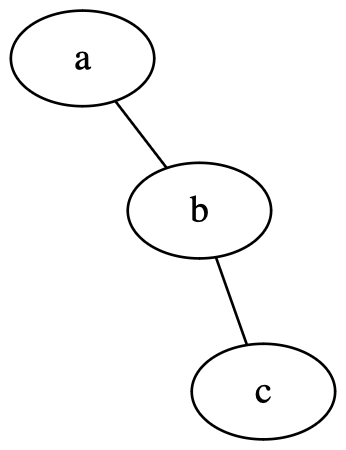
\includegraphics[width=0.7\columnwidth]{images/sparse.png}
    \caption{Sparse graph}
    \label{fig:image1}
  \end{subfigure}
  \hfill
  \begin{subfigure}[b]{0.3\columnwidth}
    \centering
    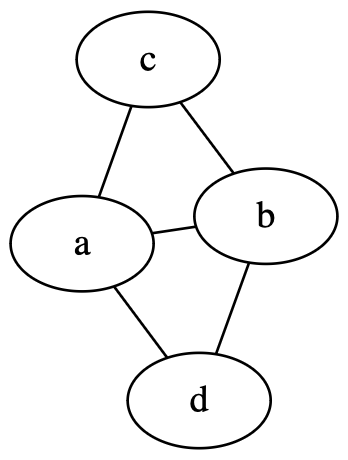
\includegraphics[width=0.7\textwidth]{images/dense.png}
    \caption{Dense graph}
    \label{fig:image2}
  \end{subfigure}
	\hfill
  \begin{subfigure}[b]{0.315\columnwidth}
    \centering
    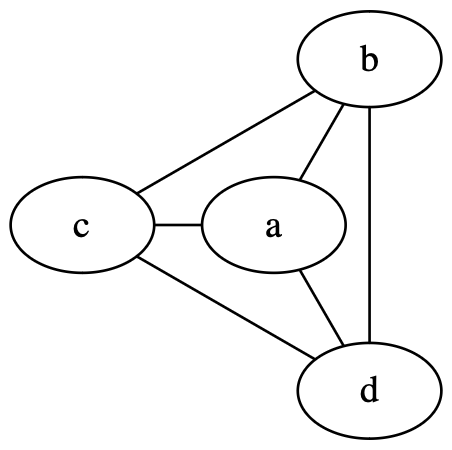
\includegraphics[width=0.9\textwidth]{images/complete.png}
    \caption{Complete graph}
    \label{fig:image3}
  \end{subfigure}
\end{figure}
}

%\hrulefill % Make distinct

\subsection*{Directed Acyclic Graphs (DAG)}
A \keydef{directed acyclic graph} is a directed graph with no cycles. DAGs are useful for representing dependencies and scheduling tasks. \\

In particular, the edges in a DAG can be interpreted as a partial order on the vertices, where $u$ precedes $v$, if $(u,v) \in E$. This partial order defines a \key{topological ordering}.\\

Some Problems become easier to solve with DAGs. \texttt{ShortestPath()} and \texttt{LongestPath()} can be solved in linear time with the help of a topological sorting.

\hfill % Prefer to shove this up

\subsection*{Topological ordering}
A \keydef{topological ordering} (also \textit{topological sorting}) of a directed acyclic graph is a partial order of the vertices, where for each vertex $u,v$ if $(u,v)\in E$, then $u$ comes before $v$ in the order.\\

The topological ordering of a DAG is \textbf{unique}, if and only if a Hamiltonian path exists.\\

If the vertices of a topological ordering $(v_1,...,v_k)$ are consecutively connected by edges, they form a \textbf{Hamiltonian path} in the graph. 

\subsubsection*{Finding a topological ordering}

A topological ordering can be found either using \texttt{Kahns algorithm}\footnote{\url{https://en.wikipedia.org/wiki/Topological_sorting\#Kahn's_algorithm}}, or by reversing the post-order of a DFS traversal. This runs in linear time.\\

\begin{figure}[H]
  \begin{subfigure}[b]{0.45\columnwidth}
    \centering
    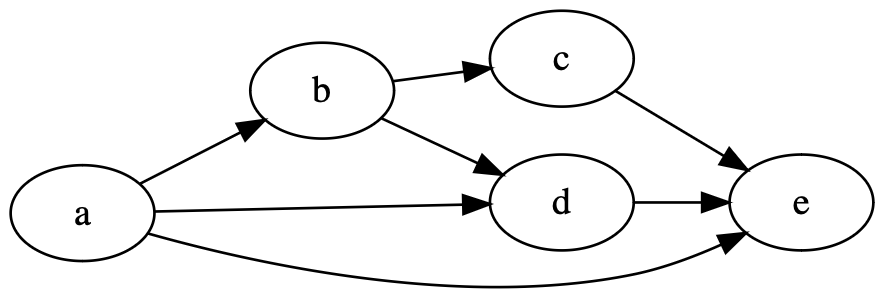
\includegraphics[width=1\textwidth]{images/dag-example-3.png}
    \label{fig:image4}
  \end{subfigure}
  \hfill
  \begin{subfigure}[b]{0.46\columnwidth}
    \centering
    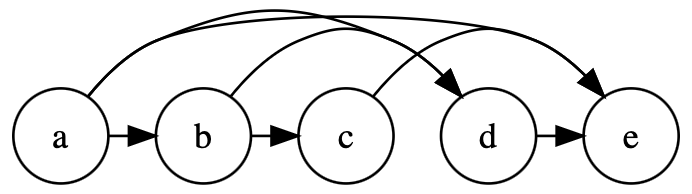
\includegraphics[width=1\textwidth]{images/dag-ordered-round.png}
    \label{fig:image5}
  \end{subfigure}
  \caption*{On the right a possible topological ordering, obtained from the reverse DFS post-order  of the left graph. }
\end{figure}

\hrulefill %TODO separator

\subsection*{Graph traversal}
\keydef{Graph traversal} is the process of visiting each vertex in a graph. \keydef{Tree traversal} is a special case, applicable to trees.

\subsubsection*{Breadth first search (BFS)}

\keydef{Breadth first search} is a graph traversal method that visits vertices with increasing depth. BFS is implemented iteratively and runs in $\oh{|V|+|E|}$.

\begin{algorithm}[H]
\caption{Breadth-First Search}
\begin{algorithmic}[1]
\Procedure{BFS}{$G, s$}
\State $Q \gets \emptyset$\Comment{Initialise empty queue}
\State Mark $s$ as active
\State $Q.\textsc{enqueue}(s)$
\While{not $Q.\textsc{isEmpty}()$}
\State $u \gets Q.\textsc{dequeue}()$
\State Mark $u$ as visited
\For{$v \in \textsc{neighbors}(u, G)$}
\If{$v$ not active and $v$ not visited}
\State Mark $v$ as active
\State $Q.\textsc{enqueue}(v)$
\EndIf
\EndFor
\EndWhile
\EndProcedure
\end{algorithmic}
\end{algorithm}

\subsubsection*{Applications of BFS}
Due to the nature of BFS, it is suitable for finding the \texttt{shortest path} in an unweighted graph. Further applications include cycle detection, checking for bipartiteness and calculating transitive closure.

\subsubsection*{Depth first search (DFS)}

\keydef{Depth first search} is a graph traversal method that explores as far as possible along each branch before backtracking. DFS runs in $\oh{|V|+|E|}$, since as it visits each vertex and edge exactly once.

\begin{algorithm}[H]
\caption{Depth-First Search (Recursive)}
\begin{algorithmic}[1]
\Procedure{DFS}{$G, s$}
\State Mark $s$ as visited \Comment{\text{\tiny{Pre-number is assigned}}}
\For{$v \in \textsc{neighbors}(s, G)$}
\If{$v$ not visited}
\State $\textsc{DFS}(G, v)$
\EndIf
\EndFor\Comment{\text{\tiny{Post-number is assigned}}}
\EndProcedure
\end{algorithmic}
\end{algorithm}

In code, DFS should be implemented iterativly. Iterative implementations are preferable due to risk of stack overflow.

\begin{algorithm}[H]
\caption{Iterative Depth-First Search}
\begin{algorithmic}[1]
\Procedure{DFS}{$G, s$}
\State $S \gets \emptyset$ \Comment{Initialise empty stack}
\State $S.\textsc{push}(s)$
\While{$S$ is not empty}
\State $u \gets S.\textsc{pop}()$
\If{$u$ not visited}
\State Mark $u$ as visited
\For{$v \in \textsc{neighbors}(u, G)$}
\State $S.\textsc{push}(v)$
\EndFor
\EndIf
\EndWhile
\EndProcedure
\end{algorithmic}
\end{algorithm}

\subsubsection*{Applications of DFS}
\begin{itemize}[noitemsep, label=-]
  \item Finding bridges and articulation points
  \item Topological sorting
  \item Finding connected components
  \item Cycle detection
\end{itemize}
\subsubsection*{Edge types}

To further understand DFS, \keydef{pre-} and \keydef{post-numbers} are introduced. The \keydef{postorder} of a DFS is given by the descending order of post-number. With the help of these numbers, one can identify special edges:
\begin{itemize}[noitemsep]
	\item \colorbox{green!30}{\textbf{Tree edge}}: In DFS tree
	\item \colorbox{blue!30}{\textbf{Forward edge}}: Skips forward in DFS tree
	\item \colorbox{violet!30}{\textbf{Back edge}}: Links back to vertex in same tree
	\item \colorbox{orange!30}{\textbf{Cross edge}}: Jumps between trees
\end{itemize}

\begin{figure}[H]
\centering
  \begin{subfigure}[c]{0.4\columnwidth}
    \centering
    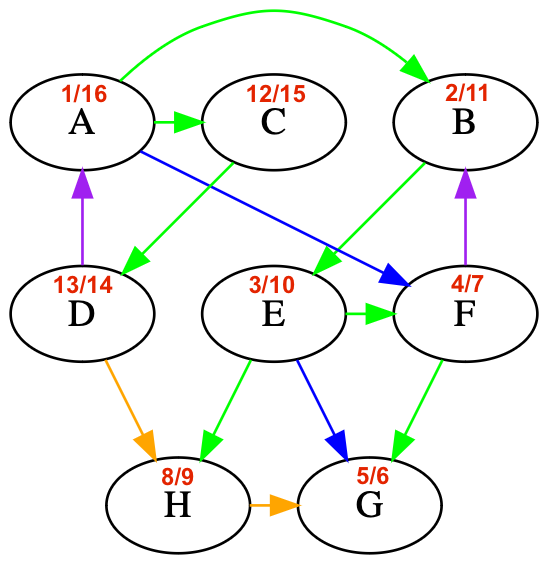
\includegraphics[width=1\textwidth]{images/edge-types-markup.png}
    \label{fig:image4}
  \end{subfigure}
  \begin{subfigure}[c]{0.58\columnwidth}
    \centering
    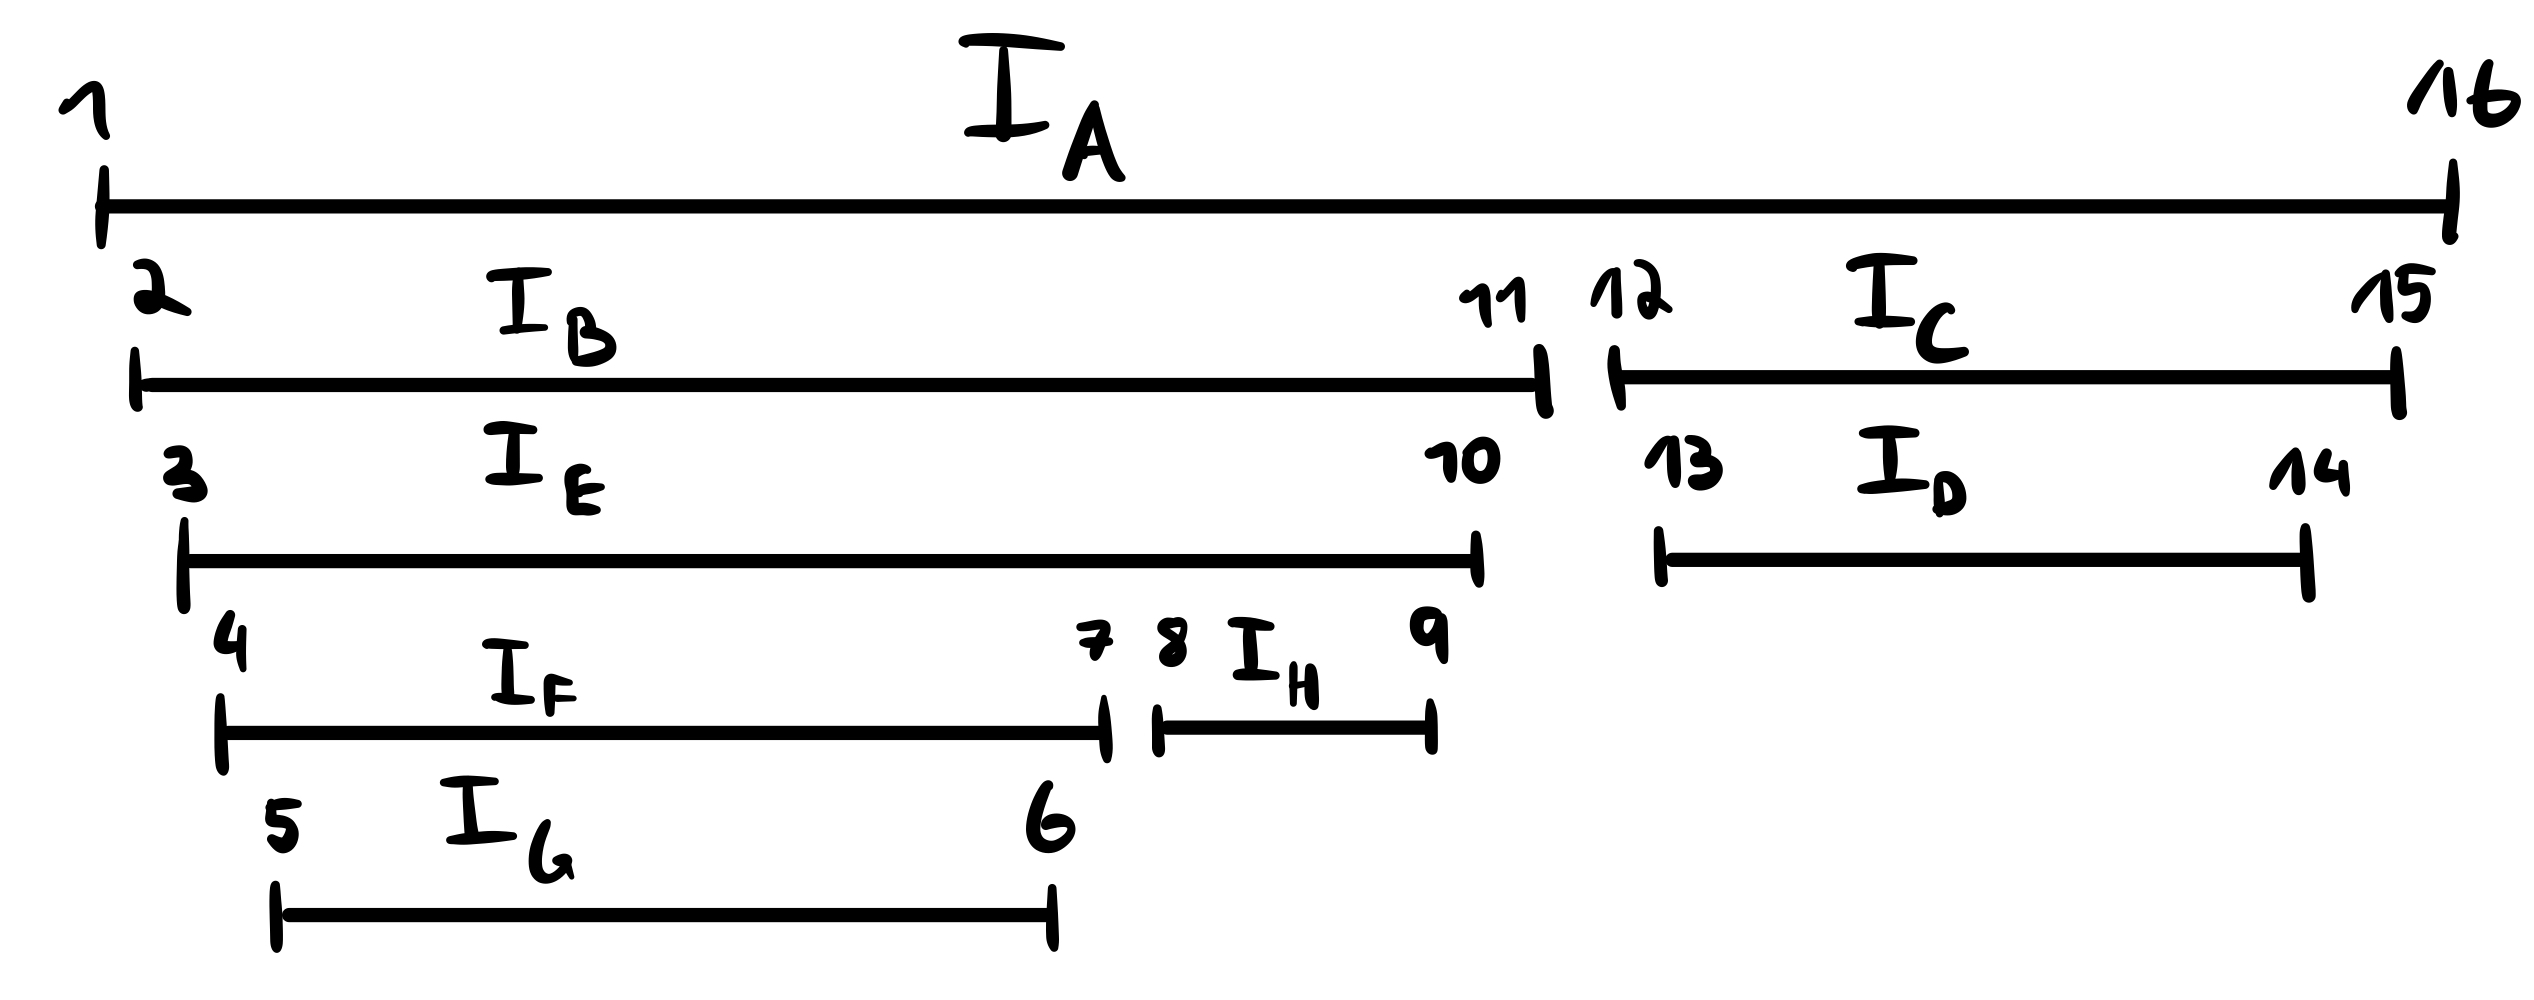
\includegraphics[width=1\textwidth]{images/interval-graph.jpeg}
    \label{fig:image5}
  \end{subfigure}
  \caption*{Graph and intervals for DFS from vertex $A$}
\end{figure}

\hrulefill % TODO separator

\subsection*{Tree traversal}
\begin{itemize}
\item \textbf{Pre-order}: Visit the current node, then recursively visit the left and right subtrees.
\item \textbf{In-order}: Recursively visit the left subtree, then visit the current node, then recursively visit the right subtree.
\item \textbf{Post-order}: Recursively visit the left and right subtrees, then visit the current node.
\end{itemize}

Each method can be implemented recursively or iteratively based on the use case.
\vfill

%%%%%%%%%%%%%%%%%%%%%%%%%%%%%%%% NEW PAGE %%%%%%%%%%%%%%%%%%%%%%%%%%%%%%%%
\newpage
\subsection*{Eulerian paths and cycles}
An \keydef{Eulerian path}\texttt{/}\keydef{Eulerian cycle} is a trail/cycle in which every edge of the graph is visited exactly once. A graph is called \keydef{Eulerian}, if and only if it contains a Eulerian cycle.\\

Eulerian paths/cycles are defined for both undirected and directed graphs. In an undirected, connected graph:
\begin{align*}
	\text{$\exists$ \key{Eulerian cycle}} \Longleftrightarrow & \text{ Every vertex has even degree} \\
	\text{$\exists$ \key{Eulerian path}} \Longleftrightarrow & \text{ $2$ or $0$ vertices have odd degree}
\end{align*}	

In a directed, weakly connected\footnote{Note that the existence of a Eulerian cycle in a directed graph implies that the graph is \textit{strongly connected}} graph:

\bigskip
$\exists$ \key{Eulerian cycle} $\Longleftrightarrow$ $\forall v\in V \operatorname{inDeg(v)}=\operatorname{outDeg(v)}$ 

\smallskip
$\exists$ \key{Eulerian path} $\Longleftrightarrow$ There exist at most 2 vertices such that $| \operatorname{inDeg(v)}-\operatorname{outDeg(v)}| = 1$. For all other vertices $\operatorname{inDeg(v)} =\operatorname{outDeg(v)}$

\subsubsection*{Constructing Eulerian cycles}
Eulerian cycles can be constructed using Hierholzer's Algorithm in $\oh{|E|}$ time.
\begin{enumerate}[noitemsep]
	\item \textbf{Iteraitvely calculate cycles}: Start from any vertex $v$ and traverse the graph, following a trail of unexplored edges until returning to $v$. 
	\item \textbf{Merge cycles}: We merge the new found cycle into the solution.
	\item \textbf{Repeat} until all cycles are merged.
\end{enumerate}
After executing the algorithm and under the assumption that the graph is Eulerian, we are left with an Eulerian cycle.

%%%%%%%%%%%%%%%%%%%%%%%%%%%%%%%% NEW PAGE %%%%%%%%%%%%%%%%%%%%%%%%%%%%%%%%
\newpage
\fancyhead[C]{Graph Theory 2}
\subsection*{Minimum Spanning trees}

A \keydef{minimum spanning tree (MST)} of a graph is a tree that spans all vertices with minimal total weight, ie. a subset of edges such that the graph is connected and the sum of weights is minimal.\\

MSTs are particularly useful for modelling network design problems, such as laying telecommunication cables or designing transportation networks.\\

By definition of a tree, a MST has $|V|-1$ edges. The MST of a graph is \textbf{unique}, if all edges have distinct weight.


\begin{figure}[H]
\centering
  \begin{subfigure}[b]{0.49\columnwidth}
    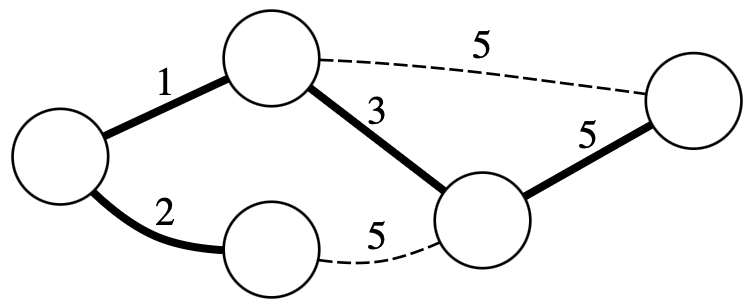
\includegraphics[width=1\textwidth]{images/mst-uniqueness-1.png}
    \label{fig:image8}
     %\caption{MST with weight 11}
  \end{subfigure}
  \begin{subfigure}[b]{0.49\columnwidth}
    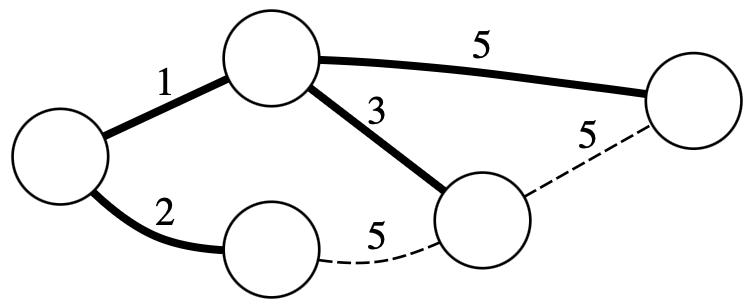
\includegraphics[width=1\textwidth]{images/mst-uniqueness-2.png}
    \label{fig:image8}
    %\caption{MST with weight 11}
  \end{subfigure}
  \caption*{Both MSTs have the same total weight}
\end{figure}



\textbf{Cycle property:} For any cycle in a graph, the maximum weight edge in that cycle cannot be part of any minimum spanning tree.\\

\textbf{Contraction:} If $T$ is a tree of MST edges, then we can contract $T$ into a single vertex while maintaining the invariant that the MST of the contracted graph plus $T$ gives the MST for the graph before contraction. ie. 

$\texttt{MST(G)} = T \cup  \texttt{MST(G contract T)}$.


\subsubsection*{Kruskal's Algorithm}
\keydef{Kruskal's algorithm} is an MST algorithm that runs in $\oh{|E| \text{log}|E|}$ time. 
\begin{enumerate}[noitemsep]
	\item Sort the edges in ascending order by edge weight
	\item For each edge $(u,v) \in E$, if $u$ and $v$ are in different components, add the edge to the MST and merge the components.
\end{enumerate}

\begin{algorithm}[H]
\caption{Kruskal's algorithm}
\begin{algorithmic}[1]
\Procedure{Kruskal}{$G$}
\State $T \gets \emptyset$ 
\State $E \gets$ edges of $G$ sorted by weight
\For{$(u,v) \in E$}
	\If{$u,v$ in different components}
		\State $T \gets T \cup \{(u,v)\}$
		
	\EndIf
\EndFor
\EndProcedure
\end{algorithmic}
\end{algorithm}

Kruskal's algorithms is very \textbf{simple} to implement. For an optimal runtime, it requires a \texttt{Union-Find} data structure to quickly find and merge components.

\vfill %TODO remove

\subsubsection*{Prim's Algorithm}
\keydef{Prim's algorithm} runs in $\oh{(|V|+|E|) \text{log}|V|}$. It is the most commonly used algorithm and is very similar to \texttt{Dijkstra's algorithm}.\\

Prim's builds a spanning tree starting from a specific vertex. In each step, it chooses the minimum edge incident to the visited vertices which connects to an unvisited vertex, and adds it to the MST.

 
 \begin{algorithm}[H]
\caption{Prim's algorithm}
\begin{algorithmic}[1]
\Procedure{Prim}{$G, s$}
\State $T \gets \emptyset$ 
\State $S \gets {s}$ \Comment{Component of $s$ in $T$}
\While{$T$ not spanning}
	\State $(u,v) \gets$ min edge to $S$, $u\in S, v \not \in S$
	\State $T \gets T \cup \{(u,v)\} $ \Comment Add $(u,v)$ to tree
	\State $S\gets S \cup \{v\}$
\EndWhile
\EndProcedure
\end{algorithmic}
\end{algorithm}
For optimal runtime, Prim's algorithm requires a \texttt{min-heap}, so that the minimum edge to $S$ can be quickly found.


\subsubsection*{Boruvka's Algorithm}

\keydef{Boruvka's algorithm} was the first MST algorithm to be discovered. It runs in $\oh{(|V|+|E|) \text{log}|V|}$. Boruvka's algorithm is particularly fast on sparse graphs and plays a key role in randomized MST-algorithms\footnote{See \url{https://en.wikipedia.org/wiki/Expected_linear_time_MST_algorithm}}.\\

 Boruvka's algorithm maintains a forest of spanning trees, where each component is initially a single vertex. In each iteration, the algorithm adds the lightest edge incident to each component to the forest. After the last iteration, the forest is a MST.

\begin{algorithm}[H]
\caption{Boruvka's algorithm}
\begin{algorithmic}[1]
\Procedure{Boruvka}{$G$}
\State $F \gets \emptyset$  \Comment{Initialise forest}
\While{$F$ not spanning}
	\State $(S_1,...,S_k) \gets$ components of $F$
	\State $(e_1,...,e_k) \gets$ minimal edges to $S_1,...,S_k$
	\State $F \gets F \cup \{e_1,...,e_k\}$
\EndWhile
\EndProcedure
\end{algorithmic}
\end{algorithm}

To achieve the optimal runtime, Boruvka's algorithm needs an efficient way to store the forest and determine the lightest edges incident to the components. This can be done using a \texttt{Union-find} data structure and a \texttt{min-heap}.

\vfill %TODO remove


\end{multicols*}
\end{document}